\chapter{Задача обратной кинематики} \label{ch:4}


\section{Введение} \label{sect:4_1}
Очень часто при решении задачи управления манипулятором возникает задача определения углов поворотов звеньев, соответствующих заданному положению. Она носит название "задача обратной кинематики". Кроме того данная проблема также возникает в компьютерной графике. Существует большое количество способов ее решения:
\begin{itemize}
	\item Использование транспонированного якобиана(Jacobian transpose)
	\item Использование псевдо-обратного якобиана(pseudoinverse Jacobian)
	\item Damped least squares
	\item Координатный спуск(Cyclic coordinate descent)
	\item Аналитическое решение
\end{itemize}

В работе рассмотрены все самые популярные методы решения задачи.


\section{Аналитическое решение} \label{sect:4_2}
Аналитическое решение очень удобно тем, что оно позволяет определить все возможные решения, время его вычисления детерминировано и сложность его расчета мала. Но существует ряд проблем, которые не позволяют его использовать для всех случаев жизни и которые породили новые численные методы решения задачи.

Во-первых аналитическое решение существует не всегда. К примеру, если манипулятор избыточен, то решений для каждой точки - бесконечное количество, соответственно так просто решение не определить.

Во-вторых его крайне сложно найти для манипуляторов с большим количеством степеней свободы. Вам понадобится много усидчивости и внимательности, чтобы правильно вывести уравнение для расчета обратной кинематики для механизма с 6 степенями свободы.

На самом деле существуют программные пакеты, такие как IKFast, которые по модели вашего манипулятора могут подобрать вам аналитическое решение. Но здесь важно понимать, что просто уравнение, а его аппроксимация полиномами высокой степени, которая в свою очередь решается численными методами, но в силу некоторых эвристических соображений, решается она очень быстро, порядка 10 мкс(требует уточнения)\cite{IKFast}. К сожалению даже для таких пакетов существуют случаи, когда решение найти невозможно.

Рассматривать геометрические способы определения аналитического решения я не буду, поскольку дело это неблагодарное, а сразу перейду к численным методам.

\section{Откуда у якобиана ноги растут} \label{sect:4_3}
Как мы могли заметить якобиан достаточно часто встречается при решении задачи обратной кинематики. Это объясняется его крайне полезными свойствами, о которых мы поговорим ниже.

Формально якобиан определяется как
\begin{align*}
	J = \frac{\partial x}{\partial q}
\end{align*} 
Согласно правилам дифференцирования сложных функций:
\begin{align*}
	J = \frac{\partial x}{\partial t} \frac{\partial t}{\partial q}		\rightarrow		\frac{\partial x}{\partial t} = J\frac{\partial q}{\partial t}
\end{align*}
Или:
\begin{align} \label{eq:4_3_1}
	\dot{x} = J\dot{q}
\end{align}
То есть якобиан связывает скорости в operational space со скоростями в joint space. Разрешив уравнение относительно $\dot{q}$, получим:
\begin{align*}
	\dot{q} = J^{-1}\dot{x}
\end{align*}

Пусть $x_{d}$ и $x_{e}$ - желаемое и текущее положение рабочего элемента соответственно. Тогда ошибка 
\begin{align} \label{eq:4_3_3}
e = x_{d} - x_{e}
\end{align}
Продифференцировав \ref{eq:4_3_3} получим,
\begin{align*}
	\dot{e} = \dot{x_{d}} - \dot{x_{e}}
\end{align*}
что с учетом \ref{eq:4_3_1} принимает вид
\begin{align*}
	\dot{e} = \dot{x_{d}} - J(q)\dot{q}
\end{align*}
Тогда выбрав скорости, как
\begin{align} \label{eq:4_3_4}
	\dot{q} = J^{-1}(q)(\dot{x_{d}} + Ke)
\end{align}
получим систему, эквивалентную
\begin{align} \label{eq:4_3_5}
	\dot{e} + Ke = 0
\end{align}
\begin{figure}[ht]
	\centering
	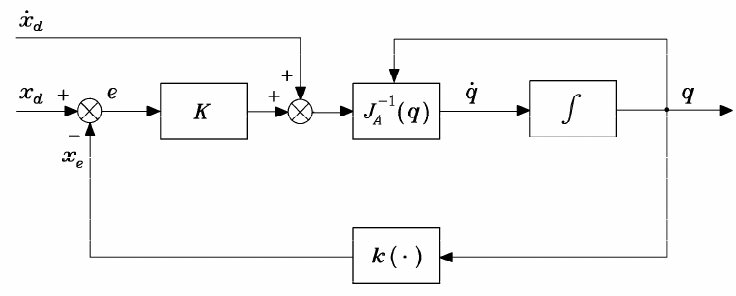
\includegraphics[scale=0.5]{IK/IK_inverse_scheme}
	\caption{Алгоритм обратной кинематики с использованием обратного Якобиана}
	\label{fig:ik_inverse_sheme}
\end{figure}
Полная схема работы алгоритма представлена на рисунке \ref{fig:ik_inverse_sheme}

Система \ref{eq:4_3_5} стабильна, если $K$ - положительно определенная матрица. Сама же матрица $K$ управляет скоростью стабилизации системы. Предполагая, что $\dot{x_{d}} = 0$ в \ref{eq:4_3_4}, получим упрощенное выражение для скоростей:
\begin{align} \label{eq:4_3_6}
	\dot{q} = J^{-1}(q)Ke
\end{align}

Уравнение \ref{eq:4_3_6} приводит нас к итеративному способу решения проблемы: будем интегрировать необходимое смещение углов с помощью метода Ньютона, то есть выбрав небольшой интервал $\Delta t$ будем на каждой итерации аппроксимировать смещение на текущей итерации как 
\begin{align*}
	\Delta q = \dot{q} \cdot \Delta t 
\end{align*}
что с учетом \ref{eq:4_3_6} принимает вид
\begin{align} \label{eq:4_3_7}
	\Delta q = J^{-1}(q)Ke\Delta t
\end{align}
и далее интегрировать полное смещение
\begin{align*}
	q(t_{k}) = q(t_{k-1}) + \Delta q
\end{align*}
На каждом этапе работы алгоритма требуется пересчитывать ошибку положений $e$, что, как следствие, требует расчета прямой кинематики $FK(q(t_{k-1}))$. Алгоритм останавливается, когда $e$ становится меньше заданного порога. 

У данного метода есть один недостаток. Уравнение \ref{eq:4_3_7} имеет решение только в том случае, если $J$ - квадратная матрица и имеет полный ранг, что на самом деле довольно редкая ситуация. Квадратным Якобиан не является, если манипулятор является избыточным, а теряет ранг в случае, когда одно или несколько звеньев двигаются сонаправленно, таким образом теряются степени свободы.


\section{Псевдо-обратный якобиан} \label{sec:4_4}
Когда манипулятор имеет избыточные звенья, то есть количество его степеней свободы больше количества переменных, которыми мы хотим управлять(к примеру манипулятор, имеющий 6 степеней свободы, в то время, как мы хотим управлять только тремя - положением без учета ориентации), то Якобиан не является квадратной матрицей, и задачу аппроксимации его обращения можно свести к проблеме линейной оптимизации с ограничениями. \cite{Bruno}

Пусть известны $v_{e}$ - скорость рабочего элемента и $J$ - Якобиан. Примем следующую квадратичную форму за функцию потерь, 
\begin{align}
	g(\dot q) = \frac{1}{2} \dot q W \dot{q}
\end{align}
которая с свою очередь должна удовлетворять ограничению \ref{eq:4_3_1}. Здесь W - любая симметричная, положительно определенная матрица размерности $[n$ $x$ $n]$. К примеру, взяв в качестве нее тензор инерции, мы минимизируем кинетическую энергию движения.

Соответствующий задаче минимизации Лагранжиан имеет вид:
\begin{align*} 
	L(\dot q, \lambda) = \frac{1}{2}\dot q W \dot{q} + \lambda(v_{e} - J\dot q)
\end{align*} 
Необходимым условием для наличия критической точки является
\begin{align*}
	\nabla L = 0
\end{align*}
откуда
\[
	\begin{cases*}
		(\frac{\partial g}{\partial \dot q})^T = \vec{0}\\
		(\frac{\partial g}{\partial \lambda})^T = \vec{0}
	\end{cases*} 
\]
Продифференцировав, получим
\[
	\begin{cases}
		\frac{\partial g}{\partial \dot q} = W\dot{q} - J^{T}\lambda = 0\\
		\frac{\partial g}{\partial \lambda} = v_{e} - J\dot{q} = 0
	\end{cases}
\]
Выразим $\dot q$ из первого уравнения
\begin{align} \label{eq:4_4_1}
	\dot q = W^{-1}J^{T}\lambda
\end{align}
 Подставив во второе уравнение, получаем
\begin{align*}
	v_{e} = JW^{-1}J^{T}\lambda
\end{align*}
Если $J$ имеет полный ранг, тогда матрица $JW^{-1}J^{T}$ обратима и мы можем вычислить множители Лагранжа:
\begin{align} \label{eq:4_4_2}
	\lambda = (JW^{-1}J^{T})^{-1}v_{e}
\end{align}
Подставив в \ref{eq:4_4_1} получим выражение для вычисления $\dot q$
\begin{align} \label{eq:4_4_3}
	\dot q = W^{-1}J^{T}(JW^{-1}J^{T})^{-1}v_{e}
\end{align}
Домножив \ref{eq:4_4_3} на $J$ легко убедиться, что ограничение \ref{eq:4_3_1} выполняется. Кроме того достаточно просто проверить, что найденное решение - точка минимума. Вторая производная функции потерь равна
\begin{align*}
	\frac{\partial^{2}g}{\partial{\dot q}^2} = W
\end{align*}
где $W$ - положительно определенная матрица, следовательно функция $g$ выпукла вниз и критическая тока является точкой минимума.
\\

Существует особый случай, когда $W$ - единичная матрица. Тогда выражение \ref{eq:4_4_3} принимает вид:
\begin{align}
	\dot q = J^{\dagger}v_{e}, \text{ где $J^{\dagger} = J^{T}(JJ^{T})^{-1}$ - правый псевдо-обратный якобиан}
\end{align}
Это решение минимизирует норму скоростей звеньев.

Кроме того псевдо-обратный якобиан имеет одно очень полезное свойство, а именно матрица $I_{n} - J^{\dagger}J$ проецирует вектор на ядро Якобиана. Если мы в качестве минимизируемого функционала примем
\begin{align*}
	g\prime(\dot q) = \frac{1}{2}(\dot q - \dot{q_{0}})^T(\dot q - \dot{q_{0}})
\end{align*}
то, проведя аналогичные вычисления, мы получим следующее решение
\begin{align}
	\dot q = J^{\dagger}v_{e} + (I_{n} - J^{\dagger}J)\dot q_{0}
\end{align}
Это означает, что если мы будем выбирать определенным образом вектор $q_{0}$, мы можем решать второстепенные задачи. К примеру, задав $v_{e}=0$, можно изменять конфигурацию манипулятора, не изменяя положения рабочего элемента, что может быть удобно для избежания препятствий. 

Обычным способом выбора является $q_{0} = k(\frac{\partial w(q)}{\partial q})^T$, где $k > 0$ - скаляр, а $w(q)$ - второстепенная целевая функция. Поскольку движение выполняется вдоль градиента $w(q)$, то движение манипулятора пытается локально максимизировать функцию, при этом не оказывая влияния на решение основной задачи.

Типичные второстепенные целевые функции \cite{Bruno}:
\begin{itemize}
	\item 	Мера управляемости,
			\begin{align*}
				w(q) = \sqrt{\det J(q)J^{T}(q)}
			\end{align*}
			максимизируя которую, манипулятор избегает вырожденных положений во время движения.
			
	\item	Расстояние до пределов джойнтов
			\begin{align*}
				w(q) = -\frac{1}{2n}\sum_{i-1}^{n}(\frac{q_{i} - \overline{q_{i}}}{q_{iM} - q_{im}})^2
			\end{align*}
			где $q_{iM}$ и $q_{im}$ - максимальные и минимальные значения углов i-го джойнта. Таким образом при движении манипулятор старается держать значения углов как можно ближе к медианам возможных принимаемых значений.
		
	\item 	Расстояние до препятствия
			\begin{align*}
				w(q) = \min ||\vec{p}(q) - \vec{o}||
			\end{align*}
			Здесь $\vec{o}$ - положение препятствия, $\vec{p}(q)$ - точка манипулятора. Таким образом во время движения манипулятор будет пытаться держать расстояние до препятствия как можно большим.
\end{itemize}

Важно заметить, что метод с использованием псевдо-обратного Якобиана не решает проблему обратимости полностью. Уравнение \ref{eq:4_4_2} имеет решение только в случае, если Якобиан имеет полный ранг, что неверно в пространстве сингулярных конфигураций. Это может привести к колебаниям вокруг решения имеющего сингулярную конфигурацию, посколько $J^{\dagger}$ принимает очень большие значения в этой области. 

\subsection{Примеры и результаты работы алгоритма}\label{subsect:4_4_1}
	Были проведены эксперименты с различными значениями точности работы(порога остановки) и скоростью схождения алгоритма.
	
	Используемые обозначения:
	\begin{itemize}
		\item $\varepsilon$ - порог остановки, рассчитывается как норма вектора ошибки.
		\item $k$ - скорость схождения. Подразумевается диагональная матрица со значениями k.
		\item $T$ - время работы алгоритма(определяется после нахождения решения).
		\item $J_{m}$ - максимальное значение нормы Якобиана(определяется после нахождения решения).
	\end{itemize}
	\bigbreak
	Параметры одинаковые для всех экспериментов:
	\begin{itemize}
		\item 	Начальное положение углов $\vec{q} = \vec{0}$.
		\item	Начальное положение рабочего элемента $\vec{s} = \{-0.4986, 0.25, 1.1428\}^{T}$.
		\item	Требуемое положение рабочего элемента $\vec{t} = \{-1.0992, 0.7642, 0.6451\}^{T}$.
	\end{itemize}
	\bigbreak
	Начальное положение имеет высокую степень сингулярности(см. рис. \ref{fig:ft_sheme1}). 
 	\bigbreak
	\textbf{Эксперимент 1:}\\
		$\varepsilon = 0.001\text{м.} = 0.1\text{см.}$\\
		$k = 0.1$\\
		$T = 502 \text{мс.}$\\
		$J_{m} = 3931$
		
		\begin{figure}[h!]
			\centering
			\includegraphics[scale=0.5]{IK/IK_pseudo_01_001/position_error}
			\caption{Ошибка положения}
			\label{fig:4_4_1}
		\end{figure}
		\begin{figure}[h!]
			\centering
			\includegraphics[scale=0.5]{IK/IK_pseudo_01_001/J_mag}
			\caption{Норма обратного якобиана}
			\label{fig:4_4_2}
		\end{figure}
		Как видно из рис. \ref{fig:4_4_2} в начале работы алгоритма Якобиан принимает очень большие значения, это связано с тем, что начальное положение манипулятора выбрано сингулярным. Это в свою очередь ведет к колебаниям в ошибке, что видно на рисунке \ref{fig:4_4_1}. Это не представляет проблемы в данном случае, посколько требуемая конфигурация не сингулярна.
		
	 	\clearpage
		\textbf{Эксперимент 2:}\\
		$\varepsilon = 0.00001\text{м.} = 0.001\text{см.}$\\
		$k = 0.1$\\
		$T = 599 \text{мс.}$\\
		$J_{m} = 3931$
		
		\begin{figure}[h!]
			\centering
			\includegraphics[scale=0.5]{IK/IK_pseudo_01_00001/position_error}
			\caption{Ошибка положения}
			\label{fig:4_4_3}
		\end{figure}
		\begin{figure}[h!]
			\centering
			\includegraphics[scale=0.5]{IK/IK_pseudo_01_00001/J_mag}
			\caption{Норма обратного якобиана}
			\label{fig:4_4_4}
		\end{figure}
		Увеличена точность работы. Графики не отличаются от полученных в первом эксперименте ничем з исключением длительности. Как видно из результатов увеличив точность в 100 раз, время работы выросло всего на 100 миллисекунд. Точности в 10мкм достаточно для решения большинства задач.
		
		\clearpage
		\textbf{Эксперимент 3:}\\
		$\varepsilon = 0.00001\text{м.} = 0.001\text{см.}$\\
		$k = 0.25$\\
		$T = 205 \text{мс.}$\\
		$J_{m} = 3931$
		
		\begin{figure}[h!]
			\centering
			\includegraphics[scale=0.5]{IK/IK_pseudo_025_00001/position_error}
			\caption{Ошибка положения}
			\label{fig:4_4_5}
		\end{figure}
		\begin{figure}[h!]
			\centering
			\includegraphics[scale=0.5]{IK/IK_pseudo_025_00001/J_mag}
			\caption{Норма обратного якобиана}
			\label{fig:4_4_6}
		\end{figure}
		Был увеличен коэффициент схождения до значения $k=0.25$, за счет чего получен большой прирост скорости работы: текущее время работы составило 205 мс., что примерно на 300 миллисекунд меньше, чем при $k=0.1$. Естественно взамен скорости мы получаем некоторые проблемы. Чем больше шаг, тем больше шанс перешагнуть через решение, таким образом возможно получить незатухающие колебания вокруг точки решения. Особенно актуальна эта проблема в сингулярных конфигурациях, когда и без того большой Якобиан умножается на высокий коэффициент. К примеру взяв $k=1$ мы никогда не получим решение для этого же случая.
		
\section{Damped least squares} \label{sect:4_5}
Как уже было сказано, уравнение \ref{eq:4_4_2} имеет решение, только если Якобиан имеет полный ранг, чего не происходит в пространстве сингулярных конфигураций. Существует другой способ обращения Якобиана, названный Damped Least-Squares pseudo-inverse. Решение слабо отличается от найденного в предыдущей главе:
\begin{align}
	J^{*} = J^{T}(JJ^{T} + k^{2}I)\\
	\dot{q} = (J^{*})^{-1}v_{e}
\end{align}
где $k$ - сглаживающий(damping) коэффициент, обеспечивающий численную стабильность вычислений при сингулярных конфигурациях. Это решение можно найти минимизировав функционал потерь\cite{Bruno}:
\begin{align}
	g''(\dot{q}) = \frac{1}{2}(v_{e} - J\dot{q})^{T}(v_{e} - J\dot{q}) + \frac{1}{2}k^{2}\dot{q}^{T}\dot{q}
\end{align}

\subsection{Примеры и результаты работы алгоритма}\label{subsect:4_5_1}
Здесь также были проведены эксперименты с различными параметрами алгоритма.

	Были проведены эксперименты с различными значениями точности работы(порога остановки) и скоростью схождения алгоритма.

Используемые обозначения:
\begin{itemize}
	\item $\varepsilon$ - порог остановки, рассчитывается как норма вектора ошибки.
	\item $\alpha$ - скорость схождения. Подразумевается диагональная матрица со значениями $\alpha$.
	\item $k$ - сглаживающий коэффициент.
	\item $T$ - время работы алгоритма(определяется после нахождения решения).
	\item $J_{m}$ - максимальное значение нормы Якобиана(определяется после нахождения решения).
\end{itemize}
\bigbreak
Параметры одинаковые для всех экспериментов:
\begin{itemize}
	\item 	Начальное положение углов $\vec{q} = \vec{0}$.
	\item	Начальное положение рабочего элемента $\vec{s} = \{-0.4986, 0.25, 1.1428\}^{T}$.
	\item	Требуемое положение рабочего элемента $\vec{t} = \{-1.0992, 0.7642, 0.6451\}^{T}$.
\end{itemize}
\bigbreak
Начальное положение имеет высокую степень сингулярности(см. рис. \ref{fig:ft_sheme1}). 
\bigbreak
\textbf{Эксперимент 1:}\\
$\varepsilon = 0.001\text{м.} = 0.1\text{см.}$\\
$\alpha = 0.1$
$k = 0.3$\\
$T = 861 \text{мс.}$\\
$J_{m} = 15.78$

\begin{figure}[h!]
	\centering
	\includegraphics[scale=0.25]{IK/IK_damped_01_001/position_error}
	\caption{Ошибка положения}
	\label{fig:4_5_1}
\end{figure}
\begin{figure}[h!]
	\centering
	\includegraphics[scale=0.25]{IK/IK_damped_01_001/J_mag}
	\caption{Норма обратного якобиана}
	\label{fig:4_5_2}
\end{figure}
Как видно из рис. \ref{fig:4_5_2} максимальное значение нормы Якобиана в сингулярной области сократилось больше чем в 200 раз по сравнению с аналогичным экспериментом, используя псевдо-обратный Якобиан. Кроме того графики нормы Якобиана и магнитуды ошибки положений на рис. \ref{fig:4_5_1} стали более гладкими, но ценой скорости работы - 800 мс. против 500 мс. с использованием псевдо-обратного Якобиана.
\bigbreak
\textbf{Эксперимент 2:}\\
$\varepsilon = 0.00001\text{м.} = 0.001\text{см.}$\\
$\alpha = 0.1$
$k = 0.1$\\
$T = 507 \text{мс.}$\\
$J_{m} = 141$

\begin{figure}[h!]
	\centering
	\includegraphics[scale=0.5]{IK/IK_damped_01_00001/position_error}
	\caption{Ошибка положения}
	\label{fig:4_5_3}
\end{figure}
\begin{figure}[h!]
	\centering
	\includegraphics[scale=0.5]{IK/IK_damped_01_00001/J_mag}
	\caption{Норма обратного якобиана}
	\label{fig:4_5_4}
\end{figure}
Сглаживающий коэффициент уменьшен в три раза с 0.3 до 0.1 и повышена точность до 10 мкм. Как видно уменьшение сглаживающего коэффициента приводит к резкому увеличению в скорости работы: хотя и была повышена точность, но время поиска решения сократилось до 507 мс., что уже почти на 100 мс. быстрее аналогичного эксперимента с использованием псевдо-обратного Якобиана.

\textbf{Эксперимент 3:}\\
$\varepsilon = 0.00001\text{м.} = 0.001\text{см.}$\\
$\alpha = 0.25$
$k = 0.1$\\
$T = 172 \text{мс.}$\\
$J_{m} = 141$

\begin{figure}[h!]
	\centering
	\includegraphics[scale=0.5]{IK/IK_damped_025_00001/position_error}
	\caption{Ошибка положения}
	\label{fig:4_5_5}
\end{figure}
\begin{figure}[h!]
	\centering
	\includegraphics[scale=0.5]{IK/IK_damped_025_00001/J_mag}
	\caption{Норма обратного якобиана}
	\label{fig:4_5_6}
\end{figure}
Увеличив коэффициент схождения до 0.25, мы получаем огромный выигрыш в скорости работы 172 мс. против 507 мс. в прошлом эксперименте. К сожалению даже со сглаживающим фактором невозможно увеличивать коэффициент до особо больших значений.

\textbf{Эксперимент 4:}\\
$\varepsilon = 0.00001\text{м.} = 0.001\text{см.}$\\
$\alpha = 1$
$k = 0.1$\\
$T = 172 \text{мс.}$\\
$J_{m} = 141$

\begin{figure}[h!]
	\centering
	\includegraphics[scale=0.5]{IK/IK_damped_1_00001/position_error}
	\caption{Ошибка положения}
	\label{fig:4_5_7}
\end{figure}
\begin{figure}[h!]
	\centering
	\includegraphics[scale=0.5]{IK/IK_damped_1_00001/J_mag}
	\caption{Норма обратного якобиана}
	\label{fig:4_5_8}
\end{figure}
То, что можно получить в сингулярной области, имея высокий коэффициент схождения показано на рисунках \ref{fig:4_5_7} и \ref{fig:4_5_8}. К счастью алгоритм все еще сходится, потому что решение находится вне пространства сингулярных конфигураций. В противном случае он мог бы никогда не найти решение, колеблясь в некоторой области вокруг него.

\section{Cyclic coordinate descent} \label{sect:4_6}